\documentclass{article}\usepackage[]{graphicx}\usepackage[]{color}
%% maxwidth is the original width if it is less than linewidth
%% otherwise use linewidth (to make sure the graphics do not exceed the margin)
\makeatletter
\def\maxwidth{ %
  \ifdim\Gin@nat@width>\linewidth
    \linewidth
  \else
    \Gin@nat@width
  \fi
}
\makeatother

\definecolor{fgcolor}{rgb}{0.345, 0.345, 0.345}
\newcommand{\hlnum}[1]{\textcolor[rgb]{0.686,0.059,0.569}{#1}}%
\newcommand{\hlstr}[1]{\textcolor[rgb]{0.192,0.494,0.8}{#1}}%
\newcommand{\hlcom}[1]{\textcolor[rgb]{0.678,0.584,0.686}{\textit{#1}}}%
\newcommand{\hlopt}[1]{\textcolor[rgb]{0,0,0}{#1}}%
\newcommand{\hlstd}[1]{\textcolor[rgb]{0.345,0.345,0.345}{#1}}%
\newcommand{\hlkwa}[1]{\textcolor[rgb]{0.161,0.373,0.58}{\textbf{#1}}}%
\newcommand{\hlkwb}[1]{\textcolor[rgb]{0.69,0.353,0.396}{#1}}%
\newcommand{\hlkwc}[1]{\textcolor[rgb]{0.333,0.667,0.333}{#1}}%
\newcommand{\hlkwd}[1]{\textcolor[rgb]{0.737,0.353,0.396}{\textbf{#1}}}%

\usepackage{framed}
\makeatletter
\newenvironment{kframe}{%
 \def\at@end@of@kframe{}%
 \ifinner\ifhmode%
  \def\at@end@of@kframe{\end{minipage}}%
  \begin{minipage}{\columnwidth}%
 \fi\fi%
 \def\FrameCommand##1{\hskip\@totalleftmargin \hskip-\fboxsep
 \colorbox{shadecolor}{##1}\hskip-\fboxsep
     % There is no \\@totalrightmargin, so:
     \hskip-\linewidth \hskip-\@totalleftmargin \hskip\columnwidth}%
 \MakeFramed {\advance\hsize-\width
   \@totalleftmargin\z@ \linewidth\hsize
   \@setminipage}}%
 {\par\unskip\endMakeFramed%
 \at@end@of@kframe}
\makeatother

\definecolor{shadecolor}{rgb}{.97, .97, .97}
\definecolor{messagecolor}{rgb}{0, 0, 0}
\definecolor{warningcolor}{rgb}{1, 0, 1}
\definecolor{errorcolor}{rgb}{1, 0, 0}
\newenvironment{knitrout}{}{} % an empty environment to be redefined in TeX

\usepackage{alltt}
\usepackage[sc]{mathpazo}
\usepackage[T1]{fontenc}
\usepackage{geometry}
\geometry{verbose,tmargin=2.5cm,bmargin=2.5cm,lmargin=2.5cm,rmargin=2.5cm}
\setcounter{secnumdepth}{2}
\setcounter{tocdepth}{2}
\usepackage{url}
\usepackage[unicode=true,pdfusetitle,
 bookmarks=true,bookmarksnumbered=true,bookmarksopen=true,bookmarksopenlevel=2,
 breaklinks=false,pdfborder={0 0 1},backref=false,colorlinks=false]
 {hyperref}
\hypersetup{
 pdfstartview={XYZ null null 1}}
\usepackage{breakurl}
\usepackage[authoryear]{natbib}
\IfFileExists{upquote.sty}{\usepackage{upquote}}{}
\begin{document}
%\SweaveOpts{concordance=TRUE}





\title{Unsupervised Document Scaling with Quanteda}


\author{Kenneth Benoit and Paul Nulty}

\maketitle

\section*{Loading Documents into Quanteda}

One of the most common tasks 

The quanteda package provides several functions for loading texts from disk into a quanteda corpus. In this example, we will load a corpus from a set of documents in a directory, where each document's attributes are specified in its filename. In this case, the filename contains the variables of interest, separated by underscores, for example:

\texttt{2010\_BUDGET\_03\_Joan\_Burton\_LAB.txt}

Quanteda provides a function to create a corpus from a directory of documents like this. The user needs to provide the path to the directory, the names of the attribute types, and the character which separates the attribute values in the filenames:

\begin{knitrout}
\definecolor{shadecolor}{rgb}{0.969, 0.969, 0.969}\color{fgcolor}\begin{kframe}
\begin{alltt}
\hlkwd{library}\hlstd{(quanteda)}
\hlstd{dirname} \hlkwb{<-} \hlstr{"~/Dropbox/QUANTESS/corpora/iebudgets/budget_2010/"}
\hlstd{attNames} \hlkwb{<-} \hlkwd{c}\hlstd{(}\hlstr{"year"}\hlstd{,} \hlstr{"debate"}\hlstd{,} \hlstr{"number"}\hlstd{,} \hlstr{"firstname"}\hlstd{,} \hlstr{"surname"}\hlstd{,} \hlstr{"party"}\hlstd{)}
\hlstd{ieBudgets} \hlkwb{<-} \hlkwd{corpusFromFilenames}\hlstd{(dirname,} \hlkwd{c}\hlstd{(}\hlstr{"year"}\hlstd{,} \hlstr{"debate"}\hlstd{,} \hlstr{"no"}\hlstd{,} \hlstr{"fname"}\hlstd{,} \hlstr{"speaker"}\hlstd{,}
    \hlstr{"party"}\hlstd{),} \hlkwc{sep} \hlstd{=} \hlstr{"_"}\hlstd{)}
\end{alltt}
\end{kframe}
\end{knitrout}



This creates a new quanteda corpus object where each text has been associated values for its attribute types extracted from the filename:

\begin{knitrout}
\definecolor{shadecolor}{rgb}{0.969, 0.969, 0.969}\color{fgcolor}\begin{kframe}
\begin{alltt}
\hlkwd{summary}\hlstd{(ieBudgets)}
\end{alltt}
\begin{verbatim}
## Corpus object contains 14 texts.
## 
##                                      Texts Types Tokens Sentences year debate
##        2010_BUDGET_01_Brian_Lenihan_FF.txt  1655   7799       390 2010 BUDGET
##       2010_BUDGET_02_Richard_Bruton_FG.txt   956   4058       222 2010 BUDGET
##         2010_BUDGET_03_Joan_Burton_LAB.txt  1485   5770       329 2010 BUDGET
##        2010_BUDGET_04_Arthur_Morgan_SF.txt  1463   6481       349 2010 BUDGET
##          2010_BUDGET_05_Brian_Cowen_FF.txt  1473   5880       262 2010 BUDGET
##           2010_BUDGET_06_Enda_Kenny_FG.txt  1066   3875       161 2010 BUDGET
##      2010_BUDGET_07_Kieran_ODonnell_FG.txt   614   2066       141 2010 BUDGET
##       2010_BUDGET_08_Eamon_Gilmore_LAB.txt  1098   3800       208 2010 BUDGET
##     2010_BUDGET_09_Michael_Higgins_LAB.txt   447   1136        49 2010 BUDGET
##        2010_BUDGET_10_Ruairi_Quinn_LAB.txt   418   1177        60 2010 BUDGET
##      2010_BUDGET_11_John_Gormley_Green.txt   363    929        49 2010 BUDGET
##        2010_BUDGET_12_Eamon_Ryan_Green.txt   482   1513        90 2010 BUDGET
##      2010_BUDGET_13_Ciaran_Cuffe_Green.txt   423   1143        48 2010 BUDGET
##  2010_BUDGET_14_Caoimhghin_OCaolain_SF.txt  1055   3654       194 2010 BUDGET
##  no      fname  speaker party
##  14 Caoimhghin OCaolain    SF
##  13     Ciaran    Cuffe Green
##  12      Eamon     Ryan Green
##  11       John  Gormley Green
##  10     Ruairi    Quinn   LAB
##  09    Michael  Higgins   LAB
##  08      Eamon  Gilmore   LAB
##  07     Kieran ODonnell    FG
##  06       Enda    Kenny    FG
##  05      Brian    Cowen    FF
##  04     Arthur   Morgan    SF
##  03       Joan   Burton   LAB
##  02    Richard   Bruton    FG
##  01      Brian  Lenihan    FF
## 
## Source:  /Users/kbenoit/Dropbox/QUANTESS/quanteda_kenlocal_gh/tutorials/scaling/* on x86_64 by kbenoit.
## Created: Wed May  7 17:12:21 2014.
## Notes:   NA.
\end{verbatim}
\end{kframe}
\end{knitrout}


In order to perform statistical analysis such as document scaling, we must extract a matrix containing the frequency of each word type from in document. In quanteda, we use the dfm function to produce such a matrix. \footnote{dfm stands for document-feature matrix --- we say `feature' instead of word, as it is sometimes useful to represent documents by features other than their word frequency.}

\begin{knitrout}
\definecolor{shadecolor}{rgb}{0.969, 0.969, 0.969}\color{fgcolor}\begin{kframe}
\begin{alltt}
\hlstd{docMat} \hlkwb{<-} \hlkwd{dfm}\hlstd{(ieBudgets)}
\end{alltt}
\begin{verbatim}
## Creating dfm: ... done.
\end{verbatim}
\begin{alltt}
\hlstd{docMat[}\hlnum{1}\hlopt{:}\hlnum{5}\hlstd{,} \hlnum{1}\hlopt{:}\hlnum{5}\hlstd{]}
\end{alltt}
\begin{verbatim}
##                                       words
## docs                                   <c3><89>ireann <c3><93> <e2><80><93>sure
##   2010_BUDGET_01_Brian_Lenihan_FF.txt               2        0                0
##   2010_BUDGET_02_Richard_Bruton_FG.txt              0        0                0
##   2010_BUDGET_03_Joan_Burton_LAB.txt                0        0                0
##   2010_BUDGET_04_Arthur_Morgan_SF.txt               0        1                0
##   2010_BUDGET_05_Brian_Cowen_FF.txt                 1        0                0
##                                       words
## docs                                   <e2><80><94> <e2><80><99>flu
##   2010_BUDGET_01_Brian_Lenihan_FF.txt             4               0
##   2010_BUDGET_02_Richard_Bruton_FG.txt            5               0
##   2010_BUDGET_03_Joan_Burton_LAB.txt             11               0
##   2010_BUDGET_04_Arthur_Morgan_SF.txt             7               0
##   2010_BUDGET_05_Brian_Cowen_FF.txt               7               0
\end{verbatim}
\end{kframe}
\end{knitrout}


We can now score and plot the documents using a statistical scaling technique, for example correspondence analysis \citep{nenadic2007}.

\begin{knitrout}
\definecolor{shadecolor}{rgb}{0.969, 0.969, 0.969}\color{fgcolor}\begin{kframe}
\begin{alltt}
\hlkwd{library}\hlstd{(ca)}
\hlstd{model} \hlkwb{<-} \hlkwd{ca}\hlstd{(}\hlkwd{t}\hlstd{(docMat),} \hlkwc{nd} \hlstd{=} \hlnum{1}\hlstd{)}
\hlkwd{dotchart}\hlstd{(model}\hlopt{$}\hlstd{colcoord[}\hlkwd{order}\hlstd{(model}\hlopt{$}\hlstd{colcoord[,} \hlnum{1}\hlstd{]),} \hlnum{1}\hlstd{],} \hlkwc{labels} \hlstd{= model}\hlopt{$}\hlstd{colnames[}\hlkwd{order}\hlstd{(model}\hlopt{$}\hlstd{colcoord[,}
    \hlnum{1}\hlstd{])])}
\end{alltt}
\end{kframe}

{\centering 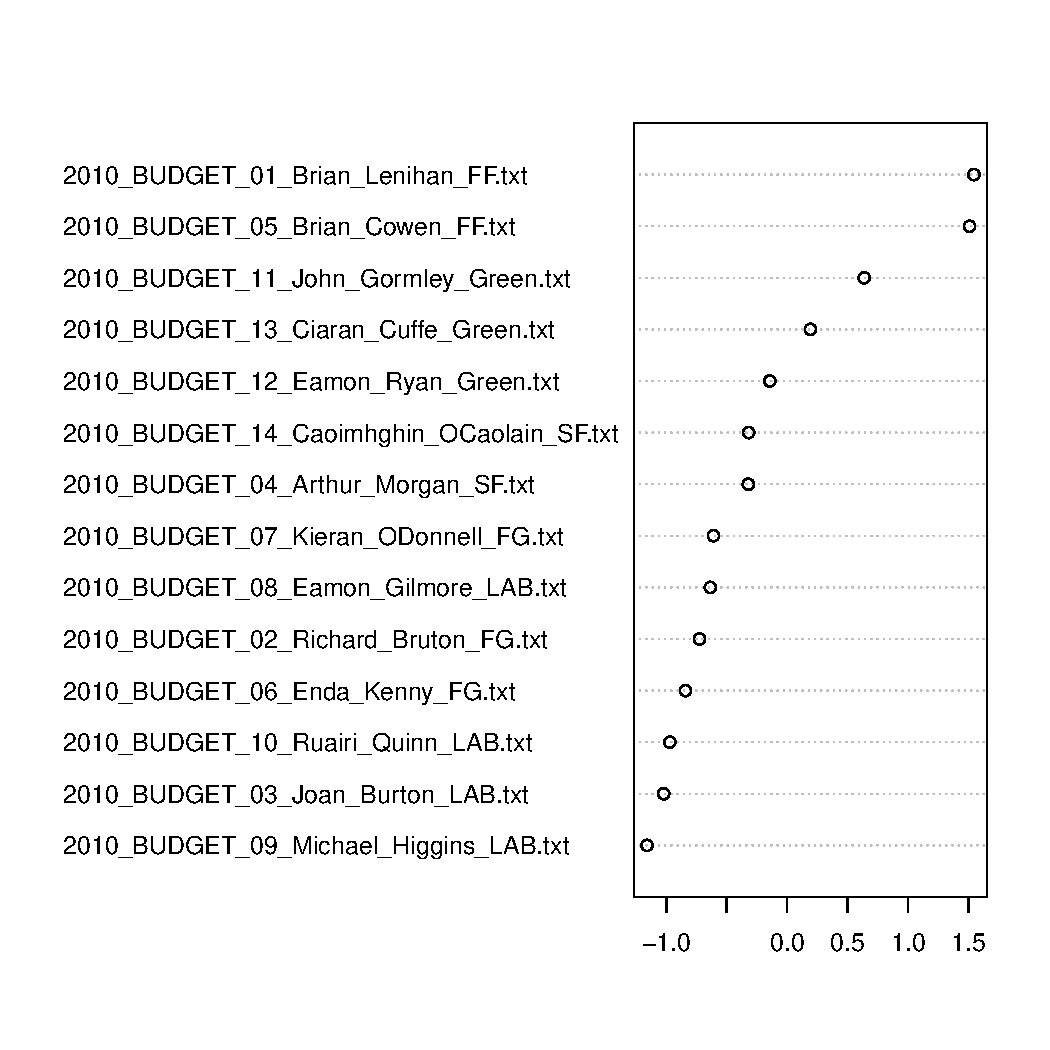
\includegraphics[width=\maxwidth]{figure/minimal-unnamed-chunk-4} 

}



\end{knitrout}


This plot indicates the position of each of the documents. We can group documents by their attribute values when creating the word-frequency matrix: 

\begin{knitrout}
\definecolor{shadecolor}{rgb}{0.969, 0.969, 0.969}\color{fgcolor}\begin{kframe}
\begin{alltt}
\hlstd{partyMat} \hlkwb{<-} \hlkwd{dfm}\hlstd{(ieBudgets,} \hlkwc{group} \hlstd{=} \hlstr{"party"}\hlstd{)}
\end{alltt}
\begin{verbatim}
## Creating dfm: ... aggregating by group: party...complete ... done.
\end{verbatim}
\begin{alltt}
\hlstd{partyMat[,} \hlnum{1}\hlopt{:}\hlnum{5}\hlstd{]}
\end{alltt}
\begin{verbatim}
##        words
## docs    <c3><89>ireann <c3><93> <e2><80><93>sure <e2><80><94> <e2><80><99>flu
##   FF                 0        0                0            5               0
##   FG                 0        0                1            9               1
##   Green              0        1                0           23               0
##   LAB                1        0                0            9               0
##   SF                 2        0                0            4               0
\end{verbatim}
\end{kframe}
\end{knitrout}


which allows us to scale according to a particular party or year, for example:

\begin{knitrout}
\definecolor{shadecolor}{rgb}{0.969, 0.969, 0.969}\color{fgcolor}\begin{kframe}
\begin{alltt}
\hlstd{partyModel} \hlkwb{<-} \hlkwd{ca}\hlstd{(}\hlkwd{t}\hlstd{(partyMat),} \hlkwc{nd} \hlstd{=} \hlnum{1}\hlstd{)}
\hlkwd{dotchart}\hlstd{(partyModel}\hlopt{$}\hlstd{colcoord[}\hlkwd{order}\hlstd{(partyModel}\hlopt{$}\hlstd{colcoord[,} \hlnum{1}\hlstd{]),} \hlnum{1}\hlstd{],} \hlkwc{labels} \hlstd{= partyModel}\hlopt{$}\hlstd{colnames[}\hlkwd{order}\hlstd{(partyModel}\hlopt{$}\hlstd{colcoord[,}
    \hlnum{1}\hlstd{])])}
\end{alltt}
\end{kframe}

{\centering 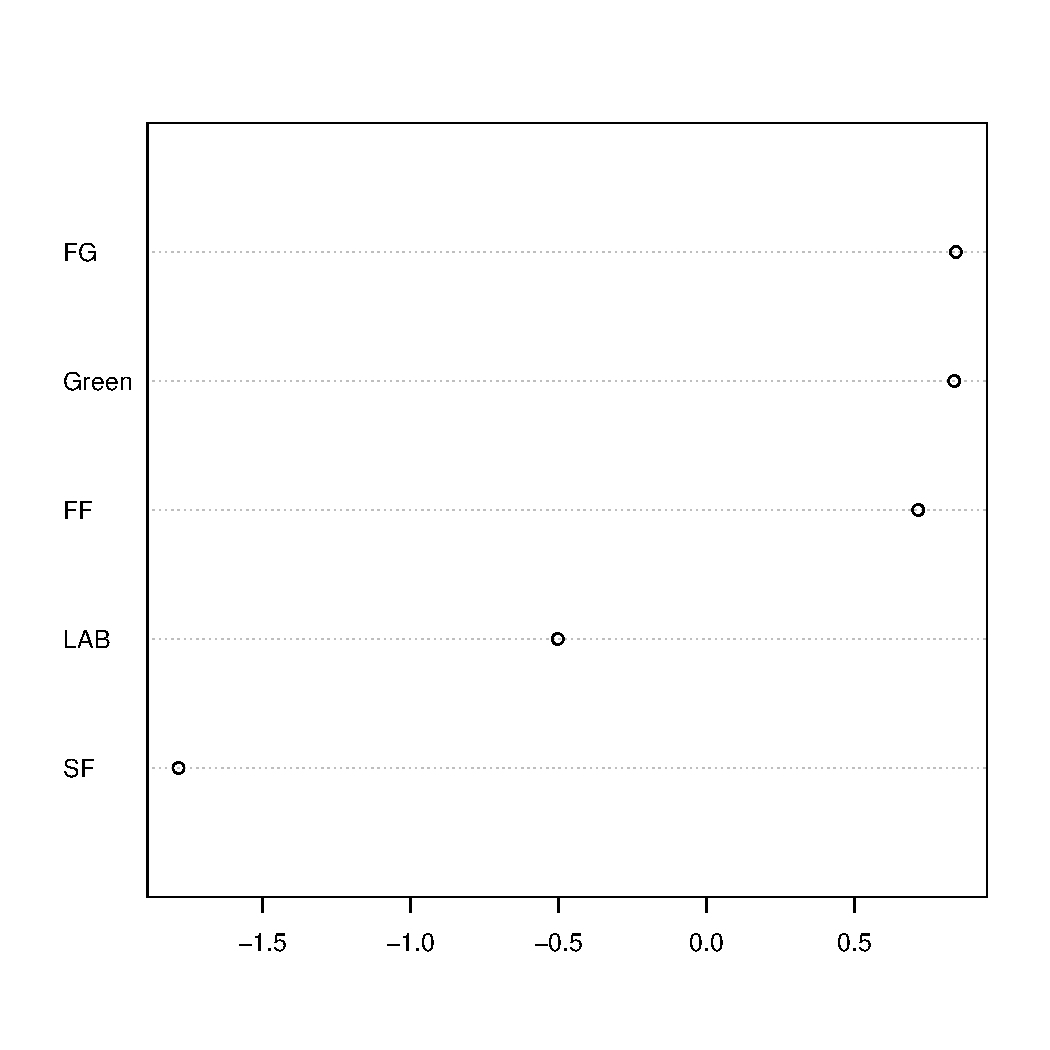
\includegraphics[width=\maxwidth]{figure/minimal-unnamed-chunk-6} 

}



\end{knitrout}

%\bibliographystyle{authordate2}
%\bibliographystyle{plain}
\bibliographystyle{plainnat}
\bibliography{scaling.bib}

\end{document}
